%! suppress = LabelConvention
\paragraph{\glspl{workpiece} und Sortierung}
\begin{itemize}
    \reqitem{1} Die \gls{anlage} kann zwischen vier Typen von \glspl{workpiece}n unterscheiden (\gls{workpiece_type}) (2, 3, 4, 5, 6)
    \begin{itemize}
        \item \gls{workpiece_flach} (3)
        \item \gls{workpiece_metall} (4)
        \item \gls{workpiece_bohrung} (5)
        \item \gls{workpiece_hoch} (6)
    \end{itemize}
    \reqitem{2} Am Ende des 2.\ \gls{belt}es sollen die \glspl{workpiece} zyklisch in folgender Reihenfolge ankommen (1, 7, 8)
    \begin{enumerate}
        \item \gls{workpiece_metall}
        \item \gls{workpiece_bohrung}
        \item \gls{workpiece_flach}
    \end{enumerate}
    \reqitem{3} \glspl{workpiece}, die nicht in die Sortierreihenfolge passen werden in eine der beiden \glspl{rampe} aussortiert (9, 10)
    \reqitem{4} Der \gls{durchsatz} an \glspl{workpiece} soll hoch sein (11)
    \reqitem{30} Aussortierung der \glspl{workpiece} soll mit \gls{weiche} funktionieren (41)
    \reqitem{38} Aussortierung der \glspl{workpiece} soll mit \gls{ejector} funktionieren (41)
    \reqitem{39} Beliebige Kombinationen der \gls{sortierer} an den beiden \glspl{anlage} sollen unterstützt werden (42)
    \reqitem{47} Wenn ein \gls{workpiece_bohrung} oder \gls{workpiece_metall} umgedreht wird, ist es ein \gls{workpiece_hoch}
\end{itemize}

\paragraph{Kapazität}
\begin{itemize}
    \reqitem{5} Bei einer vollen \gls{rampe} wird eine Warnung ausgesandt (12)
    \reqitem{6} Wenn die nächste notwendige Aussortierung aufgrund von ausgeschöpfter \glspl{rampe}kapazität
    nicht stattfinden kann, wird ein Fehler ausgesandt (und somit der Gesamtbetrieb gestoppt) (13)
\end{itemize}

\paragraph{Durchlassablauf}
\begin{itemize}
    \reqitem{7} Zuführung von \glspl{workpiece}n erfolgt durch Einlegen von \glspl{workpiece}n am Anfang von \gls{anlage} 1 (14, 15)
    \begin{itemize}
        \item Ein Unterbrechen der \gls{lb_st} signalisiert dem System das Einlegen eines \gls{workpiece}s,
        sodass der Transport dessen beginnen kann
    \end{itemize}
    \reqitem{9} Das System muss mit in beliebigem Abstand eingelegten \glspl{workpiece}n umgehen können (16, 17) %TODO Mindestabstand
    \begin{itemize}
        \item Solange der Bereich der ersten Lichtschranke frei ist, muss der Benutzer \glspl{workpiece}
        einlegen können, ohne die Korrektheit der Funktion zu gefährden
    \end{itemize}
    \reqitem{14} Der Abstand von \glspl{workpiece}n auf \gls{belt} 2 muss mindestens 25 cm betragen (18)
    \begin{itemize}
        \item Abstand muss vor der Übergabe sichergestellt werden
    \end{itemize}
    \reqitem{16} Auf dem \gls{belt} von \gls{anlage} 2 dürfen sich maximal 2 \glspl{workpiece} befinden (19)
    \reqitem{18} Falls sich bei der Übergabe zwischen den beiden \glspl{belt} ein \gls{workpiece}
    überschlägt, muss der neue \gls{workpiece_type} beachtet werden (20)
    \begin{itemize}
        \item Der Fall, dass das Teil auf die Seite fällt, sodass es wegrollen könnte, wird ausgeschlossen.
        Wenn sich das \gls{workpiece} überschlägt, ändert sich bei hohen \glspl{workpiece}n der Typ
    \end{itemize}
    \reqitem{20} \Glspl{workpiece} dürfen nicht vom \gls{belt} fallen (21)
    \reqitem{24} Beim Einlegen eines \glspl{workpiece}s in die \gls{anlage} soll dem \gls{workpiece} eine eindeutige ID zugewiesen werden(28)
    \reqitem{26} Wenn sich auf einem \gls{belt} kein \gls{workpiece} befindet, stoppt das \gls{belt}
    \reqitem{31} Wenn ein \gls{workpiece} die \gls{lb_en} von \gls{anlage} 2 erreicht,
    sollen Informationen zu diesem \gls{workpiece} auf der Konsole ausgegeben werden (22, 23, 24, 25, 26, 27)
    \begin{itemize}
        \item Zu den Informationen zählen die ID, Typ, Höhe auf \gls{anlage} 1 und \gls{anlage} 2 des \gls{workpiece}es als
        auch ein Hinweis darüber, ob sich das \gls{workpiece} überschlagen hat
    \end{itemize}
\end{itemize}

\paragraph{Bedienung durch Taster}
\begin{itemize}
    \reqitem{12} Bei Betätigung von \gls{t_start} wechselt die \gls{anlage} in den Betriebszustand (49)
    \reqitem{15} Bei \gls{longpress} von \gls{t_start} wechselt die \gls{anlage} in den Service-Modus (50)
    \begin{itemize}
        \item Anforderung für den Wechsel ist, dass die \gls{anlage} im Ruhezustand ist
    \end{itemize}
    \reqitem{17} Bei Betätigung des \gls{t_stop} wechselt die \gls{anlage} in den Ruhezustand (51, 52)
    \begin{itemize}
        \item Wenn Fehler oder Warnung vorliegen, wird stattdessen ein Fehler ausgesandt  %TODO Warnung und Fehler in glossar aufnehmen
    \end{itemize}
    \reqitem{21} Bei Betätigung des \gls{t_reset} werden sämtliche Fehler quittiert (53) %TODO mit kunden kären
    \reqitem{28} Wenn die \gls{anlage} durch \gls{estop} stillgelegt ist, kann der Betrieb durch Drücken des
    \gls{t_reset} der \gls{anlage}, an dem auch der \gls{estop} gedrückt wurde, fortgesetzt werden (56) %TODO 'fortsetzten' mit kunden kären
    \begin{itemize}
        \item Bedingung dafür: Keine \gls{estop} sind gedrückt
    \end{itemize}
    \reqitem{40} Im Service Modus führt die \gls{anlage} Kalibrierung und Selbsttests durch (50) %TODO genauer spezifizieren %TODO Modi in glossar aufnehmen
    \reqitem{41} Bei Betätigung eines \gls{estop} werden beide \glspl{anlage} angehalten (54, 55)
    \reqitem{42} Dem Benutzer werden Hinweise über die Benutzung der \gls{anlage} mithilfe der LEDs an den \gls{taster}n gegeben
    \begin{itemize}
        \item Im Betriebszustand ist die LED am \gls{t_start} an
        \item Im Ruhezustand die LED am \gls{t_stop} an
        \item Bei einem gegangenen oder bestehenden Fehler ist die LED am \gls{t_reset} an
    \end{itemize}
\end{itemize}

\paragraph{Zustandsanzeigen}
\begin{itemize}
    \reqitem{10} Im Betriebszustand leuchtet die grüne \gls{ampelled} dauerhaft (59)
    \reqitem{11} Im Service-Mode blinkt die grüne \gls{ampelled}  (60)
    \reqitem{13} Bei Warnungen blinkt die gelbe \gls{ampelled} bei der \gls{anlage}, bei der die Warnung vorliegt (61)
    \reqitem{19} Wenn im Betriebszustand keine Warnungen vorliegen, ist die gelbe \gls{ampelled} aus (61)
    \reqitem{37} Die rote \gls{ampelled} signalisiert die Fehlerzustände wie folgt (73, 74, 75, 76):
    \begin{itemize}
        \item Anstehend unquittiert wird durch schnelles Blinken (1 Hz) signalisiert (74)
        \item Anstehend quittiert wird durch dauerhaftes Leuchten(75) signalisiert
        \item Gegangen unquittiert wird durch langsames Blinken (0,5 Hz) signalisiert (z.B.\ wenn ein
        \gls{workpiece} an einer \gls{weiche} zu langsam in die \gls{rampe} geschoben wurde) (76)
        \item Steht kein Fehler an, ist die Leuchte aus (73)
    \end{itemize}
    \reqitem{45} Im Ruhezustand leuchtet die \gls{ampel} dauerhaft gelb
\end{itemize}

\paragraph{\gls{weiche}}
\begin{itemize}
    \reqitem{23} Bei Verklemmen der \gls{weiche} wird eine Warnung ausgesandt, bis das \gls{workpiece} in der Rampe ankommt (37)
    \begin{itemize}
        \item Ein \gls{workpiece} ist verklemmt, wenn das \gls{workpiece} länger als erwartet braucht, um in der \gls{rampe} anzukommen
        \item Länger als erwartet wird mit mehr als 50 Prozent der durchschnittlichen Aussortierzeit definiert
    \end{itemize}
    \reqitem{27} Die \gls{weiche} darf nicht länger als 30 Sekunden auf \gls{do_not_discard} stehen (35, 36)
    \begin{itemize}
        \item Bei minutenlangen Stromfluss wird die \gls{weiche} beschädigt
    \end{itemize}
\end{itemize}

\paragraph{\gls{recorder}}
\begin{itemize}
    \reqitem{25} Es soll eine \gls{record-fn} bereitgestellt werden, mit der ein Benutzer alle
    \glspl{event} der \gls{anlage} in ein \gls{protokoll} aufzeichnen kann (90)
    \reqitem{29} Die von der \gls{record-fn} vorgenommene Aufzeichnung soll menschenlesbar sein (91)
    \reqitem{33} Es soll eine \gls{replay-fn} bereitgestellt werden, mit der ein
    Benutzer eine zuvor aufgezeichnetes \gls{protokoll} abspielen lassen kann (93, 94)
    \reqitem{34} \glspl{protokoll} sollen per Hand angefertigt werden können (95, 96)
\end{itemize}

\paragraph{Höhenmessung}
\begin{itemize}
    \reqitem{32} Bei der Auswertung der Höhenmessung ist die durch Verkippung des Sensors entstehende Abweichung zu berücksichtigen (43, 44)
\end{itemize}

\paragraph{Fehlerumgang}
\begin{itemize}
    \reqitem{35} Nach Behebung eines Fehlers soll der Normalbetrieb fortgesetzt werden (45, 46)
    \begin{itemize}
        \item Nach Möglichkeit sollen die \glspl{belt} nicht geräumt werden
    \end{itemize}
    \reqitem{43} In den Zuständen 'bestehend\_unquittiert' und 'bestehend\_quittiert' bleiben die
    \glspl{belt} beider \glspl{anlage} stehen und \glspl{weiche} werden auf \gls{discard} gestellt
    \begin{itemize}
        \item Die Fehleranzeige mittels der \gls{ampel} ist in\refreq{37}spezifiziert
    \end{itemize}
    \reqitem{36} Fehlerzustand soll wie in Abbildung~\ref{fig:stm-fehlerzustand} beschrieben sein. (65, 66, 67, 69, 70)
    \reqitem{46} Der Fehlerzustand beider \glspl{anlage} wird wie folgt festgelegt:
    \begin{itemize}
        \item Der aktuell bestehende Fehler mit der höchsten Fehlerstufe entspricht dem Fehlerzustand beider \glspl{anlage}.
        Die Fehlerstufen lauten wie folgt:
    \begin{enumerate}
        \item Anstehend unquittiert
        \item Anstehend quittiert
        \item Gegangen unquittiert
        \item OK
    \end{enumerate}
    \end{itemize}
\end{itemize}

\begin{figure}[h]
    \centering
    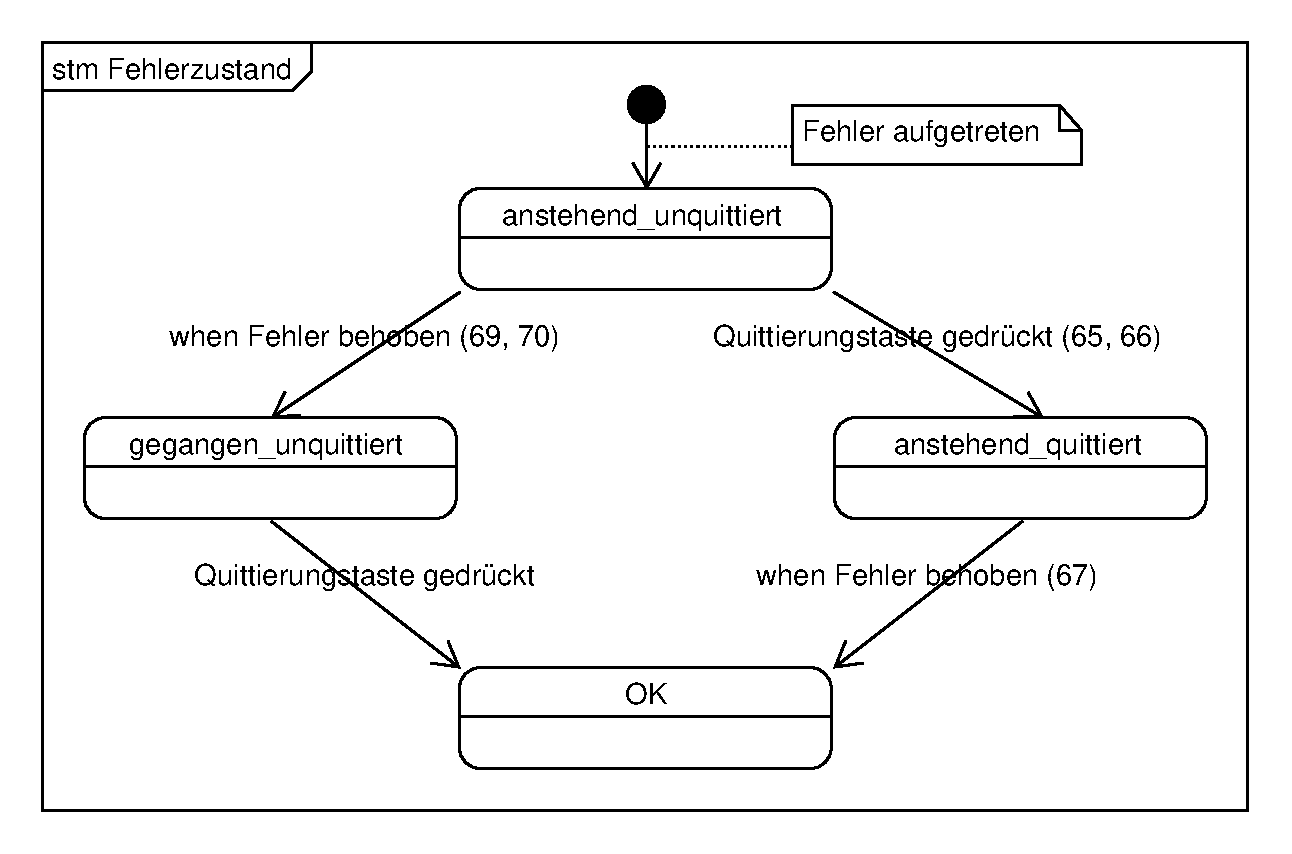
\includegraphics[scale=0.5]{../out/diagrams/stage1/req-fehlerzustand}
    \caption{REQ-36 Visualisierung des Fehlerzustandes eines einzelnen Fehlers}
    \label{fig:stm-fehlerzustand}
\end{figure}
